\section{Experiment}
In this section, we evaluate the effectiveness and efficiency of the proposed method by experimentation. To show its superiority, we apply it to test Modbus, one of the widely used ICPs. To indicate the versatility of our method, another ICP, EtherCAT, will also be used to test.

\subsection{Modbus and EtherCAT}
We choose Modbus and EtherCAT as our test targets from a variety of ICPs in the experiment. ICPs have much in common features such as a short-data frame, no encryption. They are designed to meet the real-time requirements of the control system.
\subsubsection{Modbus-TCP}
Modbus protocols have many variants, including Modbus-TCP and Modbus-UDP. Here, we use Modbus-TCP as one of the fuzzing targets, as illustrated in Fig. \ref{FigModbusFormat}. It uses master-slave communication mode, in which the master communicates with the slave by sending and receiving data frames. In the experiment, different Modbus-TCP implementations, including Modbus RSSim v8.20, Modbus Slave v6.0.2, and xMasterSlave v.156, are applied as the fuzzing targets. Finally, to better demonstrate the effectiveness of our approach, we use the serial communication mode between MCU \cite{roberts1972microprogrammed} and PC, and adopt RS485 bus \cite{feng2012design} for signal transmission to build the real Modbus network environment. The generated test cases are sent in the real environment to test the effects in practical applications.
\begin{figure}[htbp]   %  插入一栏图片
	\centering 
	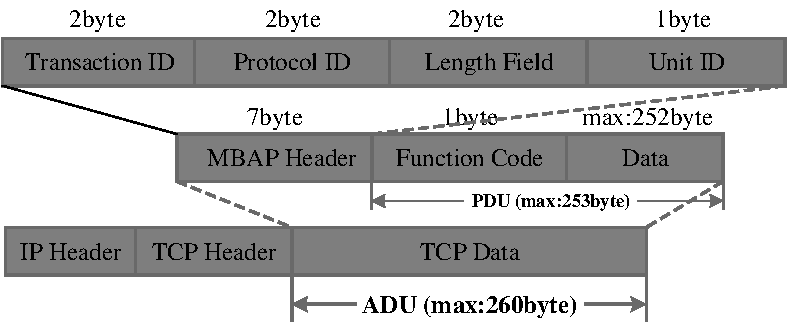
\includegraphics[width=3.2in]{FIGURE_LV/FigModbusFormat.pdf}
	\caption{Message format of Modbus-TCP}
	\label{FigModbusFormat}
\end{figure}

\subsubsection{EtherCAT}
EtherCAT offers high real-time performance and provides a master-slave communication mode among the industry devices. A typical EtherCAT network consists of one master and several slaves. The master generates datagrams and sends them to the loop network. These datagrams are reflected at the end of each network segment and sent back to the master. We test EtherCAT to prove the versatility of our method.

\subsection{Training Data}
Training data in deep learning significantly influence model training. Thus, we accurately collect and preprocess the training data. In the experiment, training data about the two industrial control protocols is collected separately.

\subsubsection{Modbus-TCP}
We use the Pymodbus \cite{Pymodbus}, a python package that implements the Modbus protocol, to generate the training data frames. Through it, we can quickly generate enough different types of data frames conveniently. Specifically, 300,000 pieces of data, including various type, are used as the training data. The data set is divided into a training set, a verification set, and a test set according to the proportion of 10-fold cross-validation.

\subsubsection{EtherCAT}
In order to capture the EtherCAT communication data, we prepare an EtherCAT based ICS. The master station is a Beckhoff \cite{Beckhoff} industrial PC, and the slave station includes EK1100 \cite{EK1100},  EL1004 \cite{EL1004} and EL2004 \cite{EL2004}. ET2000 \cite{ET2000} is used as the online Listener between the master and the slaves. The Wireshark \cite{Wireshark}, running on a computer, can fetch and display the massive communication data messages from the listener. After processing, these messages will serve as the training data for the EtherCAT protocol.
\begin{figure}[htbp]
\centering
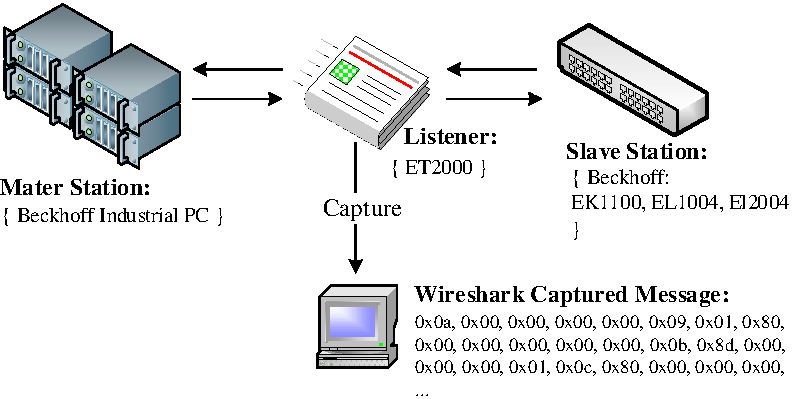
\includegraphics[width=3.3in]{FIGURE_LV/FIGURE_ETHERCAT.pdf}
\caption{EtherCAT enviroment}
\label{FIGURE_DGD}
\end{figure}

\subsection{Evaluation Setup}
\subsubsection{Experimental Environment}
We adopted Tensorflow, one of the popular deep learning framework, to implement the model architecture. To improve the training efficiency, we train the model on a Windows machine with 8 processors (Intel (R) Core (TM) i7-6700K CPU@4.00GHz) 16.0GB memory (RAM) Nvidia GeForce GTX 1080 Ti (11GB). When launching an attack, the simulators run on another machine with 4 processors (Intel (R) Core (TM) i5-5300U CPU@2.30GHz) 8.00GB memory (RAM).
\subsubsection{Model Training Setting}
As for the parameter setting, we initialize all weights from zero-centered Normal distribution with a standard deviation of 0.02. The mini-batch size is set to 256 in all models. The learning rate is set to 0.0002 in the Adam optimizer. As to the Leaky ReLU function in the discriminator model, the slope of the leak is set to 0.2. We train the models for 100 epochs and save the generator model for every ten epochs to get plentiful test cases.

\subsection{Experiment Results}
In this section, we show the experimental results in three aspects. We first present the bugs that occurred in the process of fuzzing the Modbus implementations. Then we reveal statistical results and its analysis. Lastly, to show protocol independence of our methodology in ICP’s fuzz testing, we apply it to test the EtherCAT protocol.
\subsubsection{Exception Founded}
We send the generated data frames to the aforementioned Modbus implementations which serve as Modbus slave stations. A total of 270,000 test cases generated was sent to each Modbus implementations. The effect is exciting that we successfully triggered bugs. The following describes these bugs in detail.

Much abnormal information is displayed at the console of the simulation software when the Modbus Rssim is attacked by the generated data frames. For a while, it goes crash. In detail, the software pop-ups windows prompt box after we sent about 3500 data frames, indicating that the program has crashed. We send data frames range from 3450th to 3500th to the other two simulation softwares, Modbus Slave and xMasterSlave; no abnormality occurs. This comparison shows that Modbus Rssim has some errors in the emulating Modbus-TCP protocol.

Another exception worth discussing is ``Station ID xx off-line, no response sent" in Modbus Slave. The log indicates that “Station ID 32 off-line, no response sent” after sending about 6540 data frames. But we observe that the station 32 is still online. This phenomenon makes us believe that there is an implementation flaw with the slave state judgment of Modbus Slave.

In fuzz testing the xMasterSlave, we find that the software automatically closes the window itself at times. Through the analysis of the system log, we conclude that memory overflow is the cause of the software crash, which suggests that the programmer may not consider the exception of populating with data boundary values when implementing the simulator. 

In further attacks of fuzz testing the three simulation softwares and the real environment, anomalies such as ``Using Abnormal Function Code", ``Data length Unmatched", ``Integer Overflow" and ``Abnormal Address" occur on a regular basis. We record the test cases that cause these abnormalities. All the abnormal feedbacks from the three softwares and slaves in the real environment are counted for further analysis. Other anomalies, such as ``File not Found" and ``Debugger Memory Overflow" and so on, are found only once or twice and thus are not discussed in detail.

\subsubsection{Statistical Analysis And Results}
In the study, we choose the widely used GPF \cite{demott2007revolutionizing}, GAN-based model and LSTM-based seq2seq mode as fuzzers in the control group. The systems to be tested are 3 Modbus simulation softwares, namely Modbus Slave, xMasterSlave, Pymodbus and Modbus RSSIM, and the real Modbus network environment we put up. In order to better evaluate the overall effect of the model on the protocol, we combined the experimental results of the four systems. The weights of the data obtained in these four experiments are 20\%, 20\%, 20\%, 40\% in the holistic data.

After fuzzers in the experimental group and control group are fully trained, fuzzing test is conducted by sending generated test cases through the TCP/502 port.

According to the three evaluation indicators mentioned above, we evaluate the effectiveness and efficiency of our fuzzing framework BLSTM-DCNNFuzz. Details are as follows.

\quad \textit{\textbf{a. TCRR.}}

GPF is compared with the other three fuzzing models based on depth learning, and the experimental results about $TCRR$ are shown in Fig. \ref{FIGURE_TCRR}. The horizontal line represents the performance of GPF on the systems. Due to not involving the learning process, there is no changing trend of GPF.

From the perspective of the four experiments, the performance of the TCRR indicators is: GPF $\approx$ LSTM-based model $\textless$ GAN-based model $\textless$ BLSTM-DCNNFuzz. After training more than 30 epochs, the TCRR rates of generative adversarial algorithms obviously exceed GPF algorithm, and the rising trend of rate slows down significantly after 60 epochs. The average TCRR rate of the GPF is 58. 5\%, and the TCRRs rate for generative adversarial algorithms is 75\% to 90\%. The final TCRR rate of the LSTM-based model algorithm is significantly lower than the other two groups for deep learning, which may be caused by the inability to learn the spatial characteristics of the data effectively. The function codes and parameters range of the protocol message are limited, which increases the possibility of abnormal exception in the random generation. For the generative adversarial algorithms from 50 to 100 epochs, the average TCRR rate of BLSTM-DCNNFuzz is approximately 8\% higher than GAN, which indicates that BLSTM-DCNNFuzz is more applicable to test cases generation for ICPs indirectly.
\begin{figure}[htbp]
	\centering
	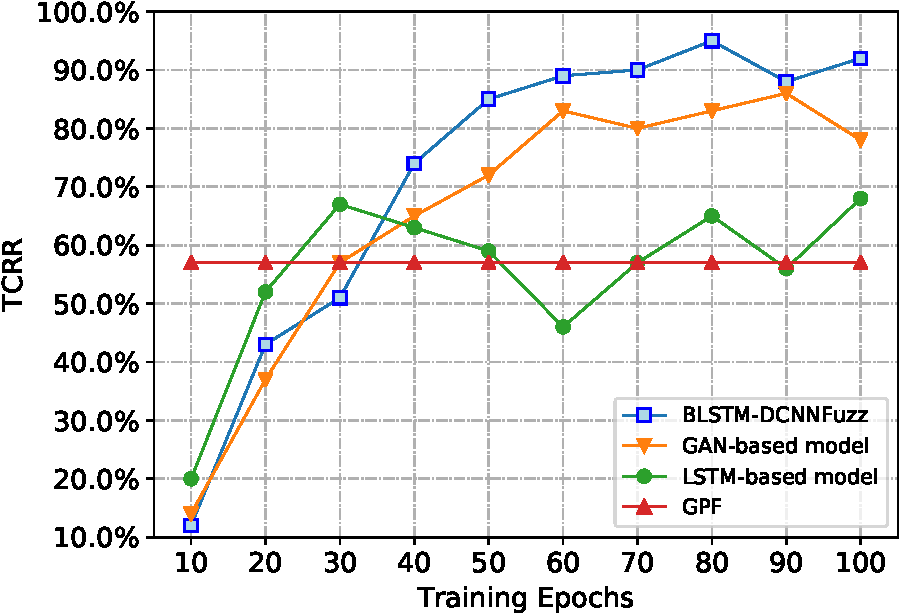
\includegraphics[width=3.36in]{FIGURE_LV/FIGURE_TCRR.pdf}
	\caption{TCRR changes with the training epochs}
	\label{FIGURE_TCRR}
\end{figure}


\quad \textit{\textbf{b. BTE.}}

When testing the Modbus implementations, we recorded triggered bugs and triggered frequency. The fuzzing test results of the four models are as follows: Table \uppercase\expandafter{\romannumeral2}. The result comparison shows our proposed methodology can trigger more vulnerabilities in higher frequency than other models, which shows the testing efficiency of BLSTM-DCNNFuzz.
\begin{table}[htbp]
	\caption{Experimental Data Comparison}
	\label{table_example}
	\centering
	\begin{tabular}{m{70pt}<{\centering}  p{30pt}<{\centering} p{30pt}<{\centering}  p{32pt}<{\centering}  p{30pt}<{\centering}}% p{40pt}p{30pt}p{40pt}p{50pt}p{40pt}
		\toprule
		\bfseries Test Model &  \bfseries Case Amount &  \bfseries Test time/h &\bfseries Bugs triggered  &\bfseries BTE Score\\
		\midrule
		BLSTM-DCNNFuzz & 18,000 & 16 & 674 & 1.37\\
		GAN-based model & 38,785 & 3 & 101 & 0.98\\
		LSTM-based model & 128,711 &  9 & 283 & 0.86\\
		GPF				 & 120,000 & 28 & 49   & 0.15 \\
		\bottomrule
	\end{tabular}
\end{table}

The concrete manifestation of BLSTM-DCNNFuzz is shown in Table \uppercase\expandafter{\romannumeral3}. 
\begin{table}[htbp]
	\caption{Triggered Bugs and Triggered Frequency of BLSTM-DCNNFuzz}
	\label{table_example}
	\centering
	\begin{tabular}{lccc}
		\toprule
		\bfseries Triggered bugs &  \bfseries Frequency (Times) & \bfseries Sent number\\
		\midrule
		Slave crash & 57 & 30,000\\
		Station ID xx off-line & 177 & 30,000 \\
		Using Abnormal Function Code & 248 & 30,000 \\
		Automatically closes the window & 73 & 30,000\\
		Data length Unmatched & 26 & 30,000 \\
		Abnormal Address & 83 & 30,000 \\
		Integer Overflow & 5 & 30,000 \\
		File not found & 3 & 30,000\\
		Debugger memory overflow & 2 & 30,000 \\
		\bottomrule
	\end{tabular}
\end{table}

\quad \textit{\textbf{c. DGD.}}
The message categories learned by GPF is constant and the coverages of different GPF are different, so it is not discussed here. The testing depth has increased as illustrated in Fig.\ref{FIGURE_TCRR} at the expense of reducing the code coverage of fuzzing test. Therefore, we need to maintain high test case diversity on the premise of attaining high TCRR rates. A total of 13 types of Modbus data frames are prepared in the original training data. When the training epochs is 10, the diversity of 3 models maintains the best. After training, some message categories are generally lost, as presented in Fig. \ref{FIGURE_DGD}. BLSTM-DCNNFuzz and LSTM-based model have good performance on maintaining basically the test case diversity, which illustrates the two models can learn the time-step dimension of protocol messages. And owing to BLSTM-DCNNFuzz containing two sub-networks for the forward and backward sequence context respectively in the BLSTM layer of BLSTM-DCNNFuzz, it is able to exploit information from both the past and the future, which performs better than LSTM-based model. Usually, the richer the data type, the higher code coverage we are likely to reach, and the stronger ability a model has to detect anomalies. Thus as presented in Table \uppercase\expandafter{\romannumeral3}, our trained model can effectively detect kinds of bugs.

\begin{figure}[htbp]
	\centering
	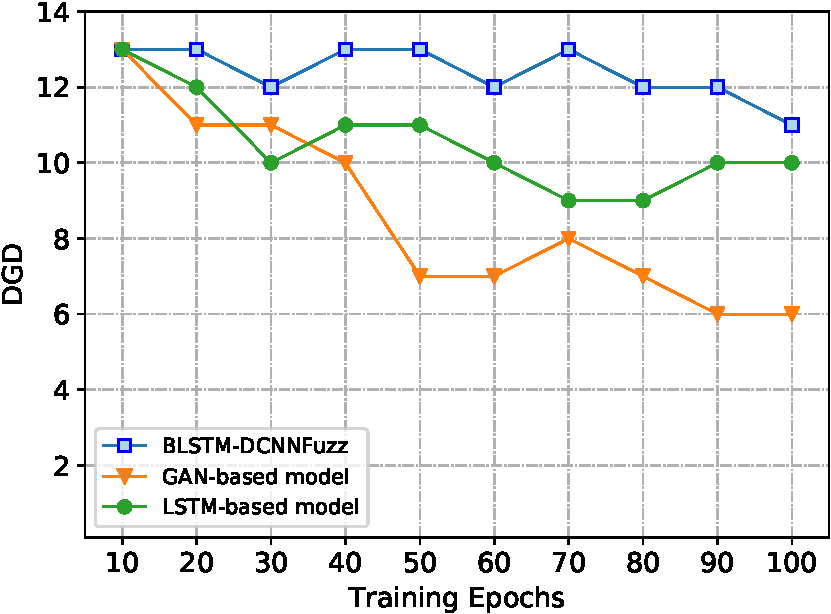
\includegraphics[width=3.3in]{FIGURE_LV/FIGURE_DGD.pdf}
	\caption{Data diversity retention}
	\label{FIGURE_DGD}
\end{figure}

\subsubsection{Applying The Method to Another ICP-EtherCAT}
To demonstrate our methodology is not just akin to a particular ICP, we apply BLSTM-DCNNFuzz to test EtherCAT, another widely used ICP. We retrain the model with captured EtherCAT data frames. With the newly trained model, massive test cases are generated expediently to detect the potential vulnerabilities of the EtherCAT protocol. The following presents the details.

\quad \textit{\textbf{a. Communication details of EtherCAT.}} EtherCAT uses a dedicated Ethernet data frame type definition to transport EtherCAT packets of Ethernet data frames. The master station initiates the communication process and controls the working status of the slave stations via process data communication. The EtherCAT slave stations extract the control information and commands from the protocol messages sent by the master station, and insert the relevant information and the collected data of the local industrial field device associated with itself. Then this Ethernet data message is transferred to the next EtherCAT slave stations. The operation repeats until all slave stations are traversed. 

\quad  \textit{\textbf{b. Detected potential vulnerabilities.}} As shown in Table \uppercase\expandafter{\romannumeral4}, we detected these potential vulnerabilities, including man-in-the-middle (MITM), MAC address spoofing, slave address attack, packet injection, working counter (WKC) attack and so on. In the experiment, we send the generated data messages $S_i$ to the slave stations and record the corresponding received message $R_i$. We get massive message pairs $<S_i, R_i>$. According to the abnormal protocol characterization above, we analyzed and compared the specified field values and obtained the following statistical results. Experiments on the EtherCAT protocol prove that our method has great versatility.
\begin{table}[htbp]
\caption{Potential Vulnerabilities and occurrences times in EtherCAT}
\label{table_EtherCAT}
\centering
\begin{tabular}{lcc}
    \toprule
    \makecell[tl]{\bfseries Potential Vulnerabilities} &  {\bfseries Occurrences times} & {\bfseries Sent Number} \\
    \midrule
    \makecell[tl]{Packet Injection Attack}  & {178 times} & 30,000 \\
    \makecell[tl]{Man In The Middle Attack} & {26 times} & 30,000 \\
    \makecell[tl]{Working Counter Attack}   & {209 times } & 30,000 \\
    \makecell[tl]{MAC Address Spoofing}  & {41 times} & 30,000 \\
    \makecell[tl]{Slave Address Attack}  & {13 times} & 30,000 \\
    \makecell[tl]{Unknown Attack}  & {597 times} & 30,000 \\
    \bottomrule
\end{tabular}
\end{table}



